\newpage % Rozdziały zaczynamy od nowej strony.
\cleardoublepage % Zaczynamy od nieparzystej strony
\pagestyle{headings}

\section{Implementacja}
W początkowej fazie projektu przetestowano wiele różnych modeli ANN w celu znalezienia odpowiedniej architektury sieci do zastosowania w przetwarzaniu obrazów. Początkowo zastosowano splotową sieć neuronową, która przy niewielkiej liczbie parametrów dawała bardzo dobre wyniki klasyfikacji odręcznie pisanych cyfr z bazy MNIST. Jednak w celu zaimplementowania algorytmu w układzie FPGA ograniczono model do postaci architektury MLP. Początkowym założeniem była możliwość zmiany parametrów sieci z~poziomu aplikacji.

\subsection{Budowa systemu}

Na początku pracy przyjęto założenie wykonywania uczenia sieci na komputerze PC z~wykorzystaniem pakietu \emph{keras}, a następnie eksport modelu w postaci plików tekstowych zawierających parametry sieci. Zbiór obrazów przedstawiających odręcznie pisane cyfry, został podzielono na testowy (10000 obrazów) oraz uczący (60000 obrazów). Ponadto system powinien umożliwiać rozpoznawanie i klasyfikację cyfr na obrazie z kamery w~czasie rzeczywistym.

\subsubsection{Schemat blokowy systemu}

System można podzielić na dwie główne części (Rys. \ref{schemat_blokowy}):
\begin{itemize}
  \item aplikacja wykorzystująca pakiet keras, uruchamiana na komputerze PC
  \item część uruchamiana na płytce Z-Turn Board
\end{itemize}

\begin{figure}[!h]
  \centering
  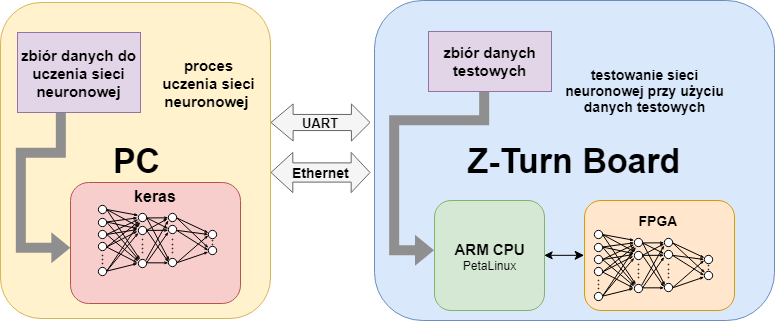
\includegraphics[width=\textwidth]{img/schemat_blokowy.png}
  \caption{Schemat blokowy systemu}
  \label{schemat_blokowy}
\end{figure}

\subsection{Wybór narzędzi}

Użycie w pracy płytki z układem Zynq determinuje użycie narzędzi wspieranych 
przez firmę Xilinx. Zdecydowano się na użycie najnowszej (w momencie rozpoczęcia 
projektu) wersji oprogramowania 2019.2. Producent zaleca \cite{VivadoGuide} instalację 
programu Vivado na jednym ze wspieranych systemów operacyjnych:

\begin{itemize}
  \item Microsoft Windows 7 SP1 Professional (64-bit), English/Japanese 
  \item Microsoft Windows 10.0 1809 Update; 10.0 1903 Update (64-bit), English/Japanese
  \item Red Hat Enterprise Workstation/Server 7.4, 7.5, and 7.6 (64-bit)
  \item SUSE Linux Enterprise 12.4 (64-bit)
  \item CentOS 7.4, 7.5, and 7.6 (64-bit)
  \item Ubuntu Linux 16.04.5 LTS; 16.04.6 LTS; 18.04.1 LTS; 18.04.02 LTS (64-bit)
  \item Amazon Linux 2 LTS (64-bit).
\end{itemize}

\bigskip
W projekcie wykorzystywane było również narzędzie Petalinux, które wymaga 
zainstalowania na maszynie z systemem operacyjnym Linux. Zgodnie z 
dokumentacją \cite{PetalinuxGuide} jest to jedna z trzech dystrybucji:

\begin{itemize}
\item Red Hat Enterprise Workstation/Server 7.4, 7.5, 7.6 (64-bit)
\item CentOS Workstation/Server 7.4, 7.5, 7.6 (64-bit)
\item Ubuntu Linux Workstation/Server 16.04.5, 16.04.6, 18.04.1,18.04.02 (64-bit)
\end{itemize}

\bigskip
Aby zapewnić poprawne działanie narzędzi oraz z racji na sporą popularność i duże 
wsparcie społeczności wybrano dystrybucję Ubuntu 18.04.02 LTS. Przy instalacji 
Petalinuxa warto również zwrócić uwagę, że zalecane jest aż 100 GB wolnego miejsca 
na dysku twardym. 

\subsection{Projekt systemu w środowisku Vivado}

Zdecydowano się na zastosowanie bloków pamięci BRAM do komunikacji pomiędzy 
blokiem IP implementowanym z użyciem HLS a procesorem. Zrzut ekranu przedstawiający 
schemat systemu w środowisku Vivado umieszczono na Rys. \ref{vivado-block-design}.
Znajduje się na nim m.in. blok IP \emph{ZYNQ7 Processing System}, przedstawiający 
procesor, oraz blok \emph{AXI Interconnect}, umożliwiający podłączenie peryferiów 
do procesora. Po podwójnym kliknięciu na blok procesora pojawia się okno, w którym
można ustawić odpowiednią konfigurację układu. 

\begin{figure}[!h]
  \centering
  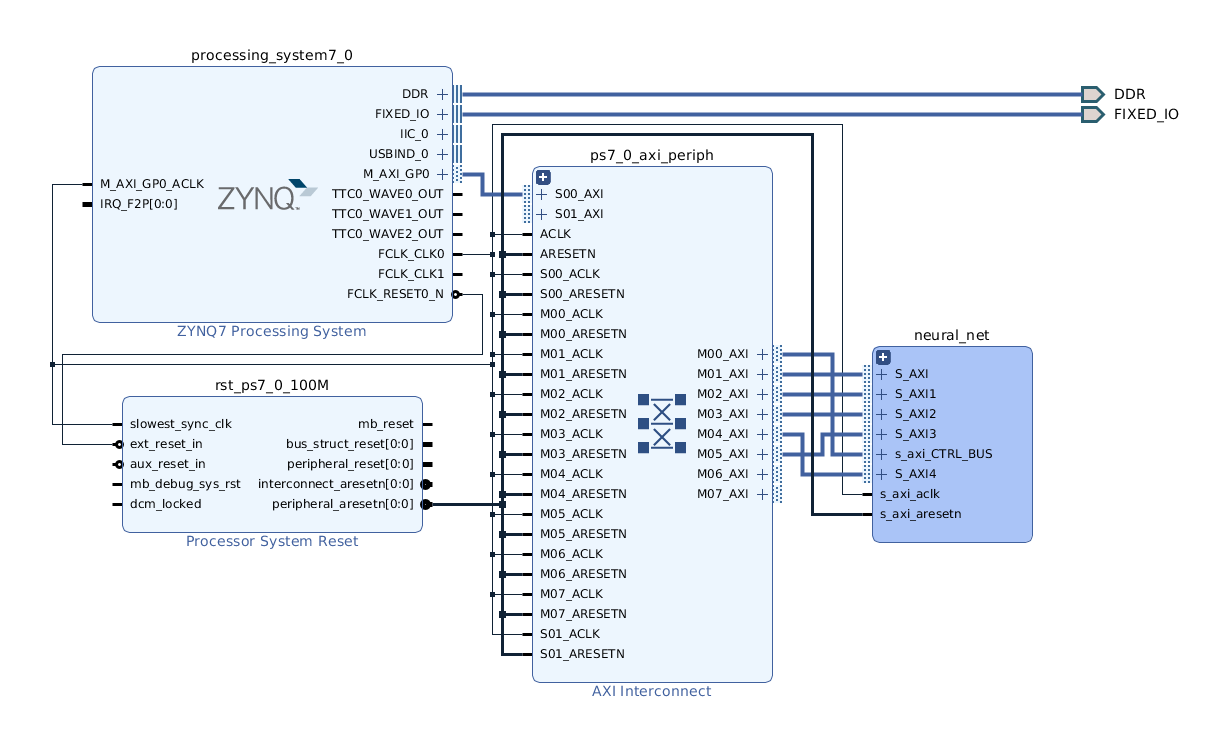
\includegraphics[width=\textwidth]{img/vivado-block-design.png}
  \caption{Zrzut ekranu przedstawiający schemat systemu w środowisku Vivado}
  \label{vivado-block-design}
\end{figure}

\subsubsection{Pamięć Block RAM}
Układy FPGA zawierają bloki dwuportowej pamięci BRAM, które można wykorzystać do komunikacji PS -- PL pomiędzy logiką programowalną (ang. PL -- \emph{Programmable Logic}) a procesorem (ang. PL -- \emph{Processing System}).
Zaletą pamięci BRAM jest możliwość równoległego dostępu do danych z dwóch niezależnych portów, jednak ilość pamięci, jaką można wykorzystać, jest mocno ograniczona. W przypadku układu Zynq-7020 znajdującego się na płytce Z-turn jest to 140 bloków po 36Kb (łącznie 4.9Mb). Pamięć BRAM umożliwia dostęp z poziomu sterownika w systemie PetaLinux do danych
przetworzonych przez blok HLS. Zdecydowano się na zastosowanie bloków pamięci BRAM do przechowywania parametrów modelu sieci oraz wejść i wyników obliczeń.

W programie Vivado pamięć alokowana jest przy użyciu bloku 
\emph{Block Memory Generator} i podłączana do procesora dzięki blokom 
\emph{AXI BRAM Controler}(Rys. \ref{vivado-block-neural}) oraz \emph{AXI Interconnect} 
(Rys. \ref{vivado-block-design}). Po odpowiednim podłączeniu bloków pamięci, w zakładce \emph{Adress Editor} można ustawić rozmiar każdego z dodanych bloków BRAM.

\begin{figure}[!h]
  \centering
  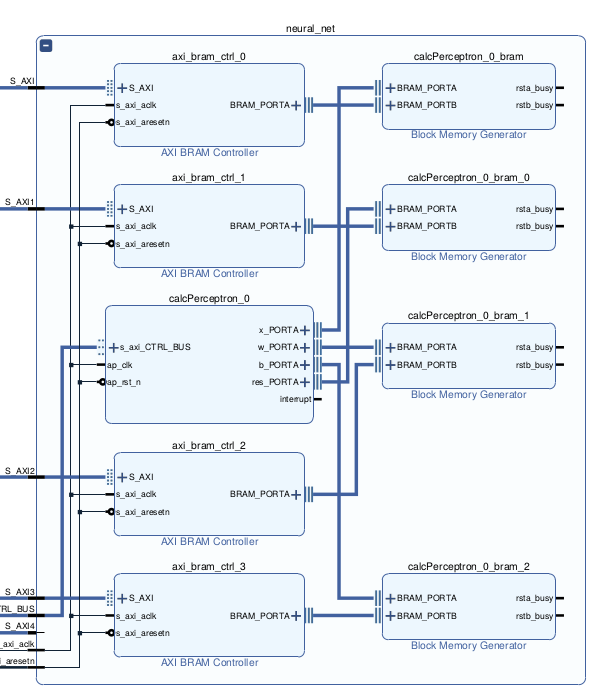
\includegraphics[width=\textwidth]{img/vivado-neuralnet.png}
  \caption{Zrzut ekranu przedstawiający szczegółowy schemat części systemu \emph{neural\_net} w~środowisku Vivado}
  \label{vivado-block-neural}
\end{figure}

\subsection{Wykorzystanie metody HLS}
Przy użyciu metody HLS możliwe jest stworzenie własnego bloku IP (ang. 
Intellectual Property), który następnie jest umieszczany w katalogu IP i można 
go wielokrotnie wykorzystać w projekcie RTL (ang. Register Transfer Level).
Do projektu z użyciem HLS (Rys.\ref{hls_design_flow}) potrzebny jest plik 
z algorytmem w języku C/C++ lub System C, plik testowy napisany w~języku C 
(ang. \emph{test bench}) oraz plik z opisem ograniczeń sprzętowych (ang. constraints).
Kolejne etapy projektu z wykorzystaniem metody HLS \cite{hlsXilinxGuide}:

\begin{enumerate}
    \item Kompilacja, wykonanie (symulacja) i debugowanie algorytmu napisanego w języku C
    \item Synteza algorytmu w języku C w implementację RTL
    \item Wygenerowanie raportu i analiza projektu (optymalizacja)
    \item Zweryfikowanie implementacji RTL
    \item Spakowanie implementacji RTL w blok IP
\end{enumerate}


\begin{figure}[!h]
  \centering
  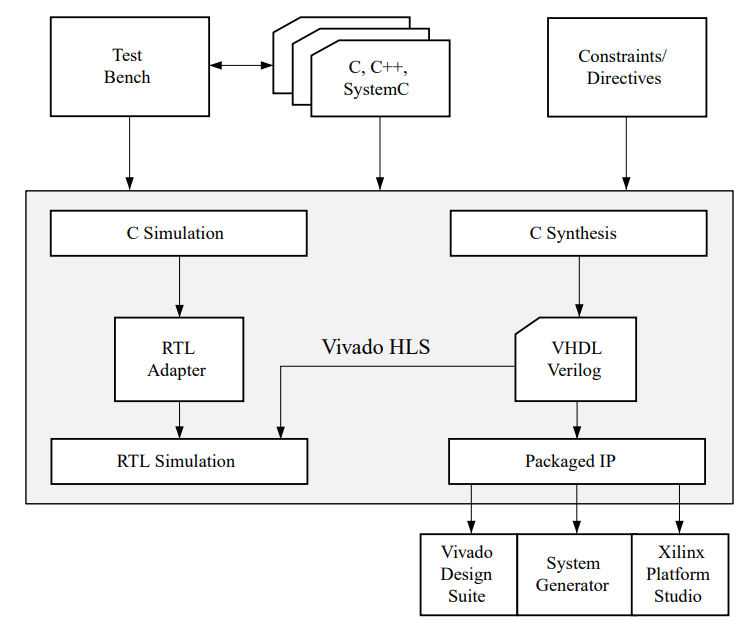
\includegraphics[width=\textwidth]{img/hls_design_flow.png}
  \caption{Proces projektowania przy użyciu metody HLS \cite{hlsXilinxGuide}}
  \label{hls_design_flow}
\end{figure}

Zastosowanie syntezy wysokiego poziomu umożliwia przeniesienie algorytmu napisanego w języku C/C++ lub System C na implementację w układzie FPGA. Dodatkową zaletą metody HLS jest dostępność bibliotek do przetwarzania 
obrazów oraz ułatwiających implementację operacji matematycznych. Podczas pracy nad projektem wykorzystano bibliotekę \emph
{<hls\_math.h>} zawierającą operacje matematyczne (np. funkcję \emph{sigmoid}), podobnie jak biblioteka \emph{<cmath.h>}. 
Obie biblioteki można wykorzystać w implementacji akceleratora HLS, jednak użycie biblioteki \emph{<cmath.h>} może powodować 
powstanie rozbieżnych wyników obliczeń podczas symulacji i syntezy.

% (Rys. \ref{hls_new_project})
Przy tworzeniu nowego projektu w Vivado HLS trzeba wybrać 
urządzenie, na którym uruchamiany będzie blok IP. Jeśli płytka nie jest widoczna na 
liście, należy dodać pliki opisujące ją w odpowiednim katalogu, gdzie zostało 
zainstalowane narzędzie Vivado HLS.  

% \begin{figure}[!h]
%   \centering
%   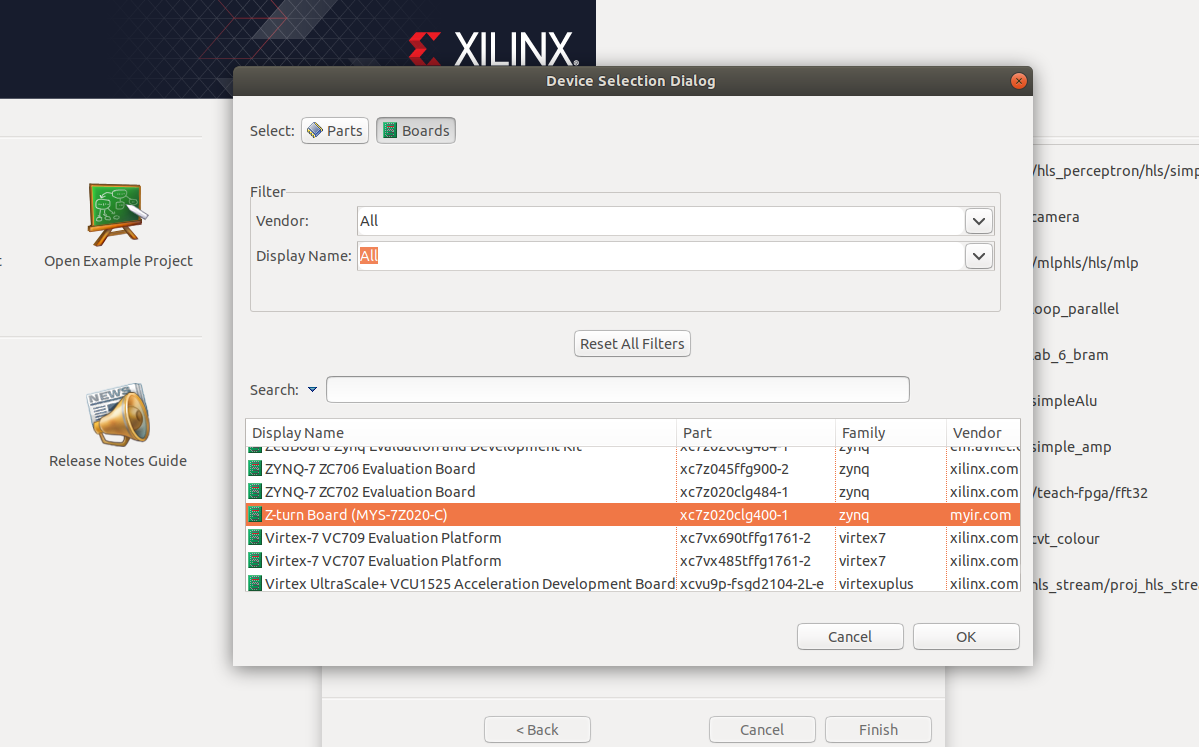
\includegraphics[width=\textwidth]{img/vivado-hls-new.png}
%   \caption{Wybór płytki podczas tworzenia projektu w Vivado HLS}
%   \label{hls_new_project}
% \end{figure}

\subsection{Optymalizacja w Vivado HLS}

Metoda HLS umożliwia optymalizację implementowanego algorytmu pod kątem zużycia zasobów układu FPGA oraz wprowadzanych opóźnień (ang. \emph{latency}). Zaimplementowany algorytm w języku C++ można optymalizować, stosując m.in. następujące dyrektywy:
\begin{itemize}
  \item rozwijanie pętli -- \emph{loop unroll}
  \item przetwarzanie potokowe -- \emph{pipeline}
  \item partycjonowanie tablic -- \emph{array partition}
  \item definiowanie zależności -- \emph{dependence}
\end{itemize} 
Wykorzystanie tych metod umożliwia poprawę wydajności implementacji, jednak zazwyczaj wiąże się ze zużyciem większej ilości zasobów logiki programowalnej. W narzędziu Vivado HLS dyrektywy są implementowane przy użyciu \emph{pragm}, umieszczanych w odpowiednie miejsce w kodzie. Po wprowadzeniu zmian w kodzie i przeprowadzeniu syntezy narzędzie Vivado HLS generuje raport, który umożliwia wstępne sprawdzenie efektów optymalizacji. Na Rys. \ref{hls-report} przedstawiono raport po przeprowadzeniu syntezy implementacji, w której wszystkie pętle są zależne od parametrów modelu ustawionych z poziomu aplikacji. Stąd, widoczne w raporcie znaki zapytania w tabeli \emph{Latency}, gdyż opóźnienia zależą od parametrów funkcji akceleratora. Poza opóźnieniami warto przeanalizować ilość zużytych zasobów, a w szczególności pole \emph{Utilization}, informujące o procentowym zużyciu zasobów. Dodatkowo przydatnym narzędziem jest \emph{Schedule Viewer} dostpęny w zakładce \emph{Analysis} (Rys. \ref{scheduler}), umożliwiający analizę czasu wykonania instrukcji w kolejnych cyklach zegara.

\begin{figure}[!h]
  \centering
  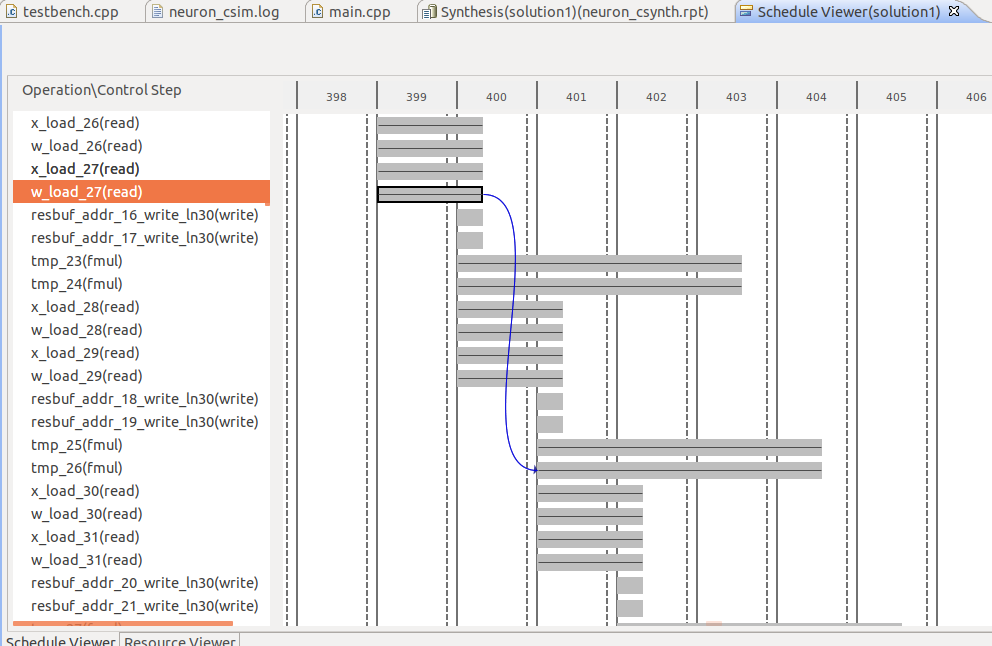
\includegraphics[width=\textwidth]{img/scheduler.png}
  \caption{Widok narzędzia Schedule Viewer w Vivado HLS}
  \label{scheduler}
\end{figure}


W prezentowanym przypadku analiza na poziomie implementacji HLS nie była możliwa ze względu na zbyt dużą ilość zmiennych parametrów, ustalanych na etapie uruchomienia aplikacji. Przeprowadzono testy z poziomu aplikacji w systemie Petalinux dla różnych modeli sieci. Na tym etapie projektu w celu pełnego skorzystania z metod optymalizacji w Vivado HLS, podjęto decyzję o wybraniu modelu sieci, który zostanie na stałe zaimplementowany, bez możliwości zmiany liczby neuronów i warstw sieci.


\begin{figure}
  \centering
  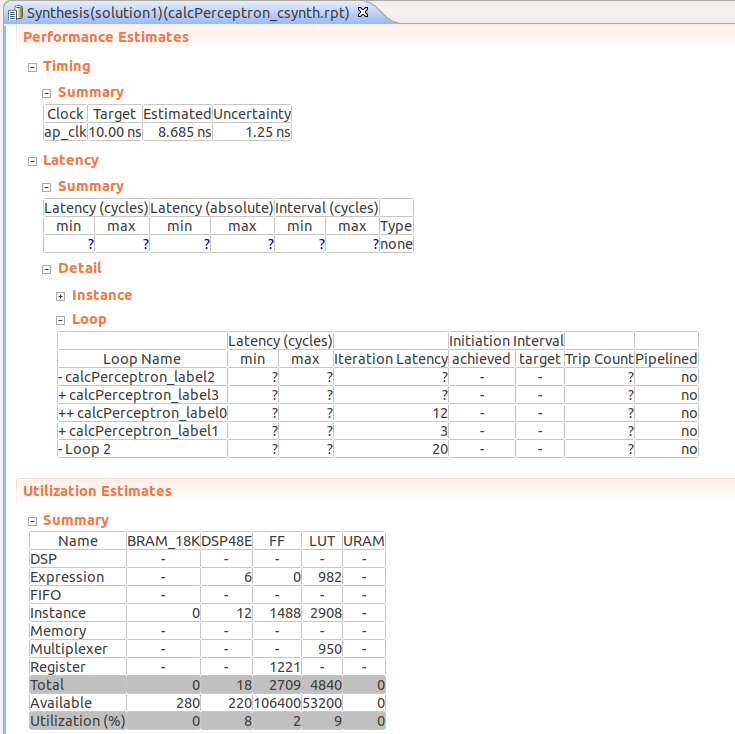
\includegraphics[width=\textwidth]{img/hls-report.png}
  \caption{Raport po przeprowadzeniu syntezy w Vivado HLS}
  \label{hls-report}
\end{figure}

\subsubsection{Rozwijanie pętli}

Każda pętla w danej implementacji wprowadza pewne opóźnienie (ang. \emph{latency}) w~działaniu kodu. Przykładowo, gdy pętla składa się z 4 iteracji, nie ma możliwości, żeby kod wykonał się szybciej niż w 4 cyklach zegara. Aby przyspieszyć wykonanie kodu, można zastosować rozwijanie pętli (ang. \emph{loop unrolling}. W przypadku rozwijania całej pętli wszystkie iteracje danej pętli wykonują się równolegle. W przypadku pętli o wielu iteracjach i ograniczonych zasobach można zastosować rozwijanie częściowe. Użytkownik podaje wartość współczynnika, która informuje o tym, ile iteracji pętli rozpocznie wykonanie jednocześnie.

\subsubsection{Pipeline}
Zastosowanie dyrektywy \emph{pipeline} umożliwia wykonanie jednej iteracji funkcji lub pętli przed zakończeniem wykonywania poprzedniej. Argumentem dyrektywy PIPELINE jest \emph{II} (ang. \emph{Initiation Interval}), który informuje o tym, ile taktów zegara będzie pomiędzy rozpoczęciem wykonywania kolejnych instrukcji. W zależności od poziomu skomplikowania implementacji i zależności zmiennych w danej pętli, osiągnięcie \emph{II=1} może wymagać wprowadzenia zmian w kodzie lub zastosowania dodatkowych dyrektyw. Wpływ zastosowania dyrektywy \emph{pipeline} na ilość cykli zegara potrzebnych do wykonania pętli zaprezentowano na Rys. \ref{pipeline}.

\begin{figure}[!h]
  \centering
  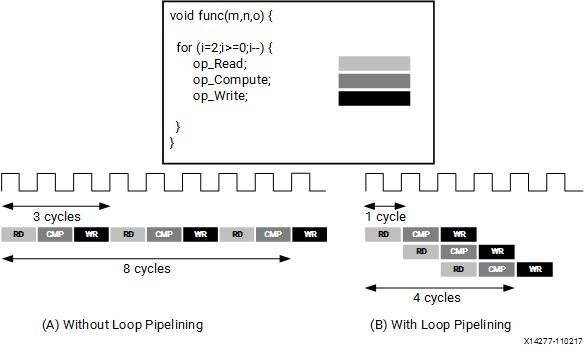
\includegraphics[width=0.9\textwidth]{img/pipeline.png}
  \caption{Wynik zastosowania dyrektywy \emph{pipeline} w celu optymalizacji pętli, (A) -- bez dyrektywy \emph{pipeline},  (B) -- z zastosowaniem dyrektywy \emph{pipeline} \cite{pipeline}}
  \label{pipeline}
\end{figure}

\subsubsection{Dyrektywa \emph{Dependence}}

Kompilator Vivado HLS automatycznie wykrywa zależności pomiędzy zmiennymi wewnątrz pętli i pomiędzy różnymi iteracjami pętli (ang. \emph{loop-carry dependence}) \cite{hls-pragmas}. W~niektórych złożonych implementacjach może dojść do nieprawidłowego zinterpretowania zależności. W tym wypadku można zastosować dyrektywę DEPENDENCE na zmiennej znajdującej się wewnątrz danej pętli lub funkcji, podając jako parametr wartość \emph{false}.

\subsubsection{Partycjonowanie pamięci}

W przypadku posiadania w kodzie zmiennych tablicowych, zawierających dużo elementów, można zastosować dyrektywę ARRAY PARTITION. Powoduje to rozdzielenie pamięci do większej liczby bloków, których liczba zależy od wartości parametru \emph{factor} podanego w dyrektywie. Partycjonowanie pamięci umożliwia zwielokrotnienie dostępu (zapis i odczyt) do pamięci. W przypadku zastosowania dyrektywy:
\begin{verbatim}
  #pragma HLS ARRAY_PARTITION variable=w block factor=4 dim=1
\end{verbatim}
pamięć przypisana do zmiennej \emph{w} zostanie podzielona na 4 bloki zawierające $\frac{N}{4}$ elementów, gdzie N jest początkowym rozmiarem tablicy. 

\subsubsection{Arytmetyka zmiennoprzecinkowa}

Kolejną metodą optymalizacji w metodzie HLS jest zamiana arytmetyki zmiennoprzecinkowej (ang. \emph{floating point}) na zapis 
stałoprzecinkowy (ang. \emph{fixed\ point}). Narzędzie Vivado HLS zawiera bibliotekę \emph{ap\_fixed.h}, która ułatwia 
definiowanie zmiennych o~wybranym typie stałoprzecinkowym oraz implementowanie operacji matematycznych z~użyciem różnych 
typów stałoprzecinkowych. Programista może wybrać liczbę bitów przeznaczonych na część całkowitą i ułamek danej zmiennej, co umożliwia odpowiednie dopasowanie typu zmiennych do wykonywanych obliczeń. Dzięki temu możliwe jest zmniejszenie zużycia zasobów oraz akceleracja obliczeń przy zachowaniu założonej precyzji. Przy dobieraniu liczby bitów w typie stałoprzecinkowym należy wziąć pod uwagę zakres wartości, jakie będzie w stanie przechowywać, co bywa skomplikowane w~przypadku złożonych algorytmów z dużą ilością operacji matematycznych. 


\subsection{Zbiór danych wejściowych}

W procesie uczenia oraz testowania poprawności działania modelu sztucznej 
sieci neuronowej wykorzystano zbiór odręcznie pisanych cyfr MNIST 
(ang. THE MNIST DATABASE of handwritten digits)\cite{lecun-mnisthandwrittendigit-2010}. Jest to baza 60000 obrazów do 
przeznaczonych do uczenia sieci oraz 10000 do walidacji. Każdy obraz przedstawia jedną cyfrę w formacie 28$\times$28 pikseli. 
Fragment zbioru MNIST przedstawiono na Rys. \ref{mnist-set}.

\begin{figure}[!h]
  \centering
  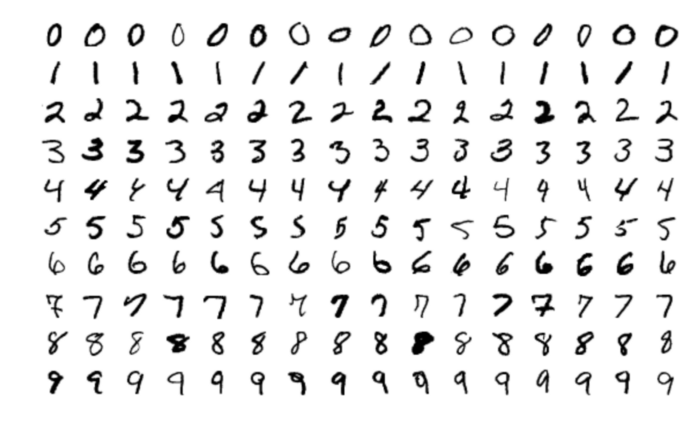
\includegraphics[width=\textwidth]{img/mnist.png}
  \caption{Fragment zbioru odręcznie pisanych cyfr MNIST \cite{lecun-mnisthandwrittendigit-2010}}
  \label{mnist-set}
\end{figure}

\subsection{Opracowanie modelu ANN}

Przy projektowaniu algorytmu ANN bardzo ważnym aspektem jest odpowiednie dopasowanie modelu do danych wejściowych. 
Najczęściej odbywa się to poprzez wielokrotne testowanie systemu dla różnych parametrów sieci. W tej pracy początkowym 
wyborem była architektura MLP. Dane wejściowe w postaci obrazów 28$\times$28 pikseli są konwertowane na tablicę 784 wartości z przedziału od 0 do 1. Fragment kodu przedstawia Listing \ref{lst:mlp}. Model zawiera następujące warstwy:
\begin{itemize}
  \item warstwę wejściową (784 wejścia)
  \item warstwę ukrytą (16 neuronów)
  \item warstwę wyjściową (10 neuronów).
\end{itemize}

% Dla dłuższych numerów linii
% potrzebne jest większe wcięcie.
\begin{addmargin}[10mm]{0mm}
  \begin{lstlisting}[
      label=lst:mlp,
      language=python,
      numbers=left,
      firstnumber=55,
      caption={Implementacja modelu ANN MLP z jedną warstwą ukrytą},
      aboveskip=0pt
  ]
model = Sequential()
model.add(Flatten())
model.add(Dense(16, use_bias=True, activation='sigmoid'))
model.add(Dense(num_classes, use_bias=True, activation='sigmoid'))

  \end{lstlisting}
  \end{addmargin}

\subsubsection{Uczenie Sztucznej Sieci Neuronowej}
Podczas uczenia i testowania modelu użyto zbioru MNIST, który zaimportowano, wykorzystując
funkcję z pakietu keras. Dokonano uczenia sieci neuronowej przy użyciu zbioru 60000 
obrazów i testowania modelu, podając na wejście sieci 10000 obrazów. Osiągnięto 
dokładność na poziomie 94,97\%. Na Rys. \ref{keras-accuracy1} przedstawiono, jak zmieniała się dokładność (ang.\emph{accuracy}) w kolejnych epokach dla zbioru uczącego i walidacyjnego.

\begin{figure}[!h]
  \centering
  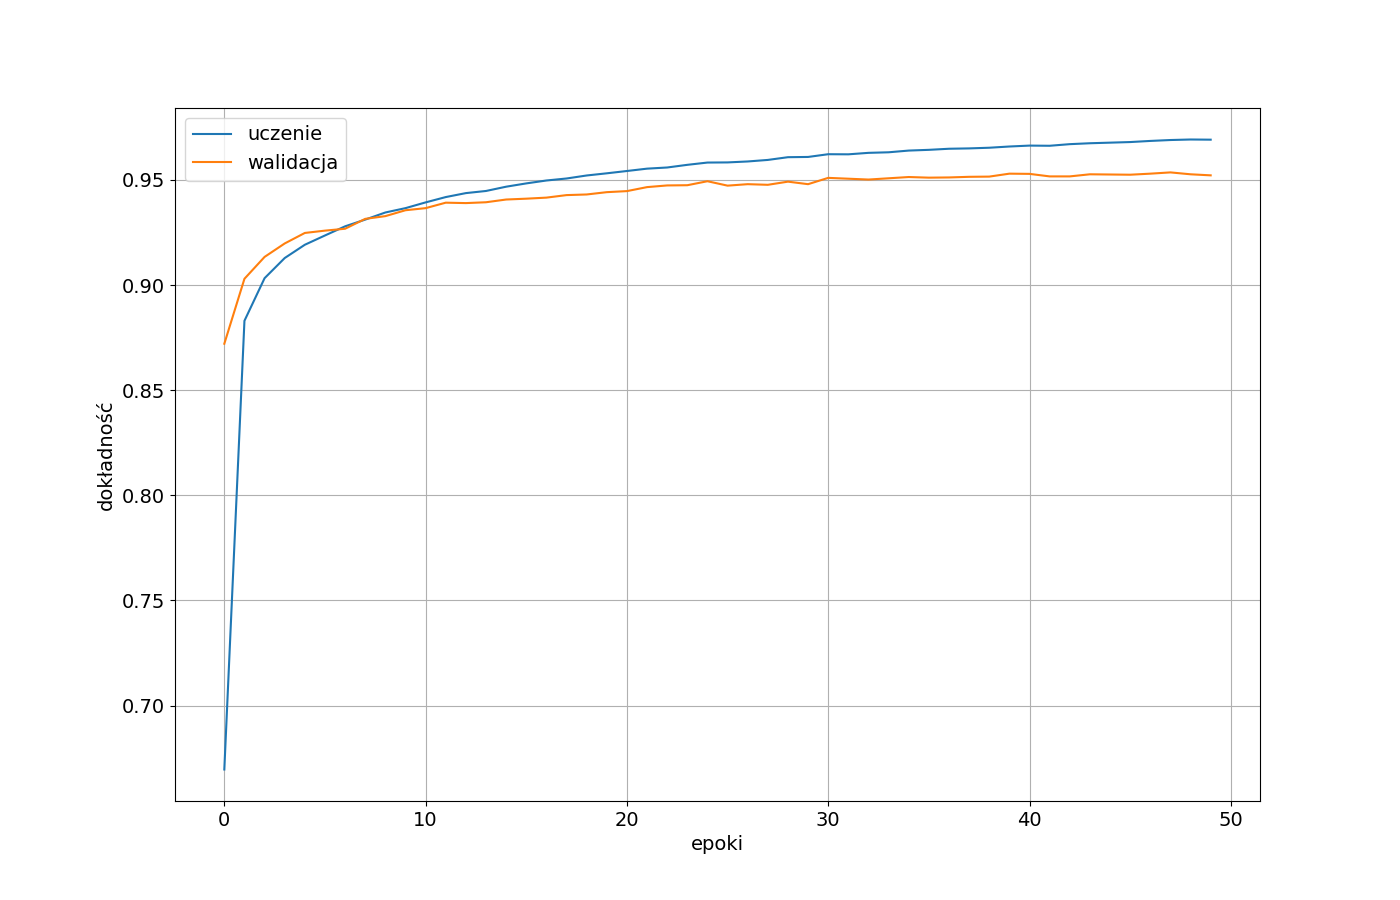
\includegraphics[width=\textwidth]{img/keras-accuracy1.png}
  \caption{Wykres zmian dokładności w kolejnych epokach -- ANN z jedną warstwą ukrytą}
  \label{keras-accuracy1}
\end{figure}

% Wprowadzenie zmian w postaci dodania większej ilości neuronów w warstwie ukrytej nie 
% powodowały zwiększenia dokładności, więc podjęto decyzję o wykorzystaniu tego modelu 
% w dalszej części projektu. 

\subsubsection{Implementacja modelu przy użyciu narzędzia Vivado HLS}

Korzystając z narzędzia Vivado HLS, napisano program w języku C++ implementujący 
zaprojektowany wcześniej model sieci. W procesie uczenia ustalono wartości wag i 
biasów. Dwa główne pliki projektu w narzędziu Vivado HLS to core.cpp, zawierający 
implementację algorytmu ANN oraz test\_core.cpp, który służy do przetestowania
algorytmu po przeprowadzeniu syntezy (ang. \emph{test bench}).   
Pliki zawierające wartości wejściowe, a także wagi i biasy są importowane 
do programu test\_core.cpp. 

Pierwszym etapem jest Symulacja C, która jest wstępną weryfikacją poprawności
algorytmu. Do przeprowadzenia symulacji wykorzystano dane wyeksportowane przy użyciu 
skryptu \emph{keras2fpga.py} i zapisane w plikach hls\_biases.h, hls\_weights.h oraz 
hls\_input.h. Wynikiem symulacji jest plik .log, w którym można znaleźć informacje o
tym, jak przebiegało wywołanie testowanych funkcji.\ref{hls_design_sim}
Symulację w języku C wykonuje się dużo szybciej niż późniejszą symulację RTL, więc
stosuje się ją jako pierwszy etap przed podjęciem dalszych kroków, które zajmują 
więcej czasu.

\begin{figure}[!h]
  \centering
  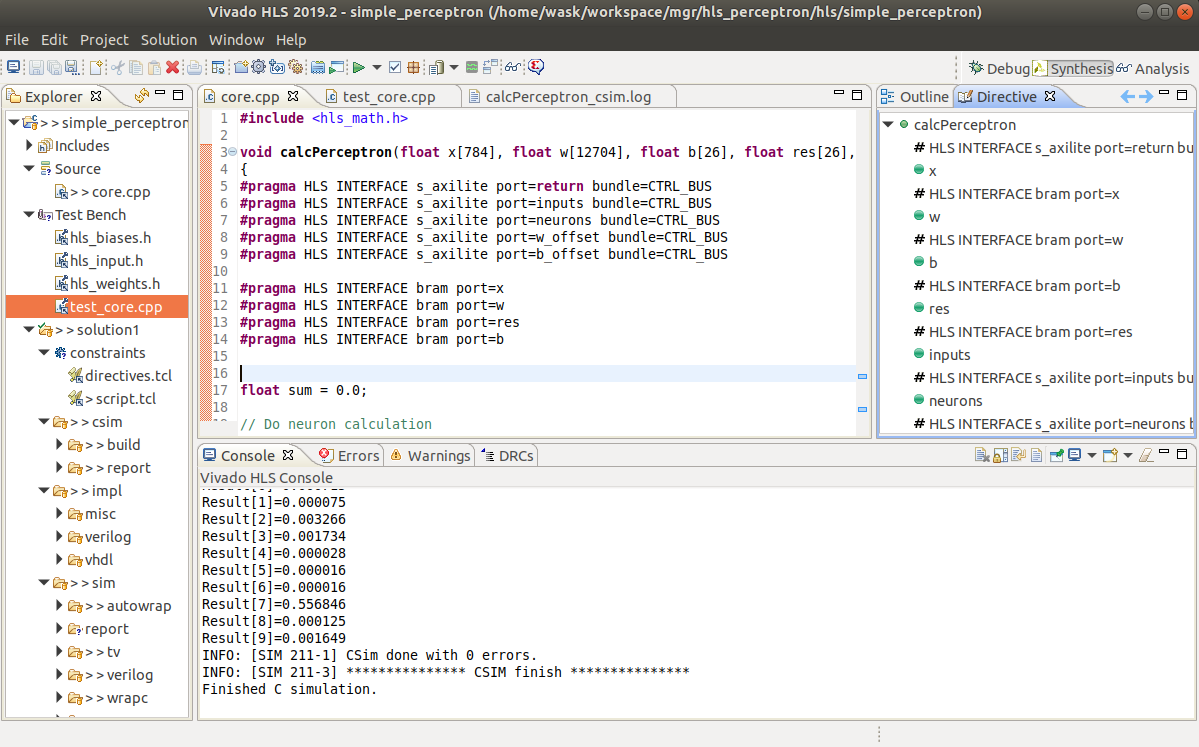
\includegraphics[width=\textwidth]{img/vivado_hls_sim.png}
  \caption{Wynik poprawnie przeprowadzonej symulacji w Vivado HLS}
  \label{hls_design_sim}
\end{figure}


Następnie wykonywana jest synteza oraz kosymulacja, umożliwiająca 
weryfikację poprawności syntezy. Ponadto narzędzie generuje raport, który przedstawia
informacje na temat zużycia zasobów i opóźnień czasowych. Po prawidłowym 
przeprowadzeniu kosymulacji należy użyć opcji \emph{Export RTL}, co umożliwia 
dodanie nowego bloku IP do projektu w narzędziu Vivado.

\subsection{Synteza projektu w narzędziu Vivado}

Aby przetestować działanie nowego bloku IP w narzędziu Vivado HLS, należy dodać i~odpowiednio podłączyć blok do 
schematu blokowego (ang. \emph{Block Design}) w narzędziu Vivado. Następnie należy sprawdzić, czy urządzenia zostały 
właściwie zaadresowane w~zakładce \emph{Adress Editor} i wprowadzić ewentualne zmiany. Gotowy projekt można poddać 
automatycznej weryfikacji za pomocą funkcji \emph{Validate Design} i uruchomić syntezę i implementację. Po poprawnie 
przeprowadzonej implementacji narzędzie umożliwia otwarcie realizacji sprzętowej projektu (opcja \emph{Open Implemented 
Design}). Zakładka \emph{Timing} (Rys. \ref{impl_design_vivado}) umożliwia sprawdzenie, czy w zaimplementowanym 
projekcie zostały spełnione wymagania czasowe, a w oknie \emph{Device} można zweryfikować jakie zasoby zostały użyte w~implementacji.

\begin{figure}[!h]
  \centering
  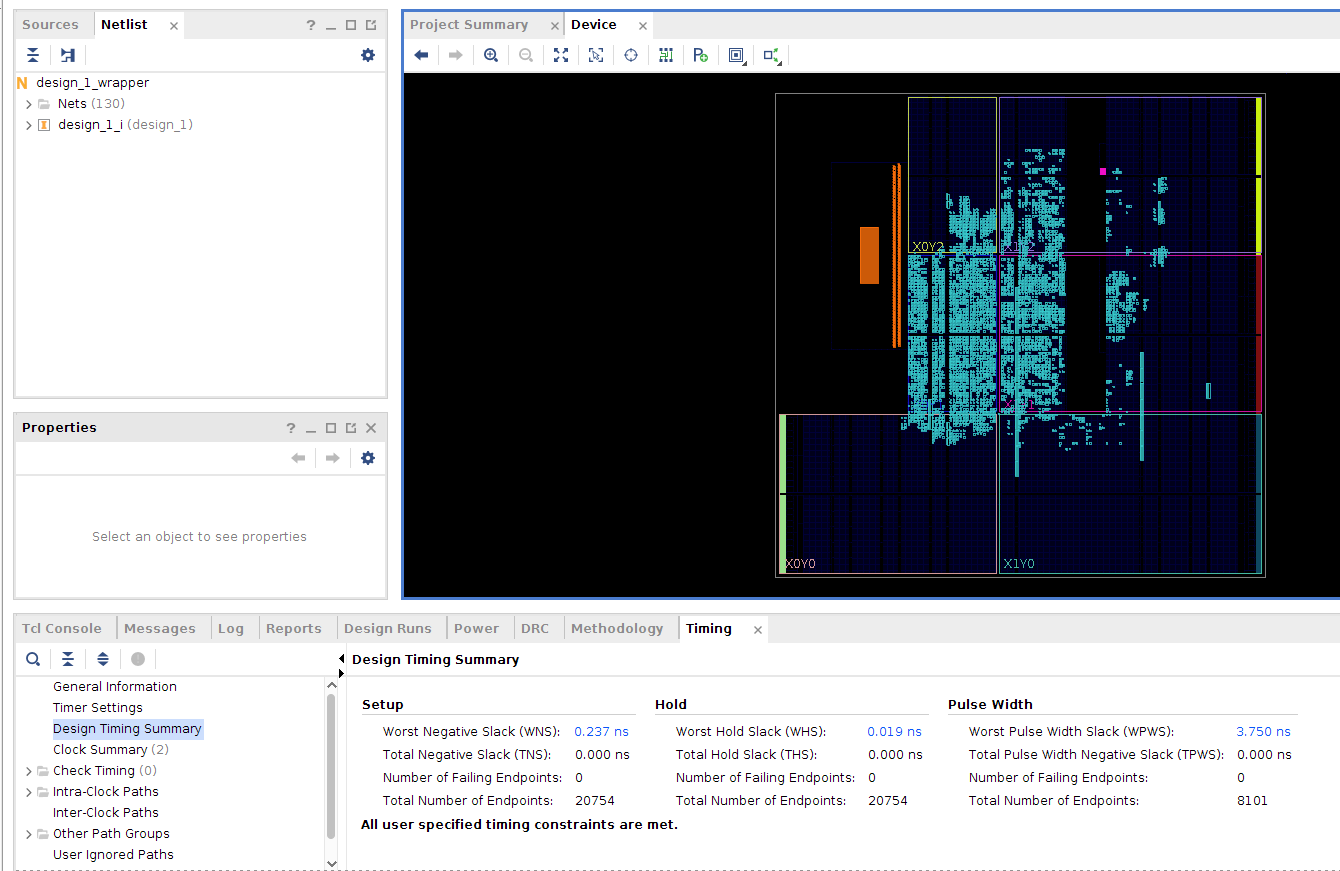
\includegraphics[width=\textwidth]{img/impl-design-vivado.png}
  \caption{Wynik poprawnie przeprowadzonej implementacji w narzędziu Vivado}
  \label{impl_design_vivado}
\end{figure}

Następnym krokiem jest wygenerowanie \emph{Bitstreamu} i eksport sprzętu w postaci pliku z rozszerzeniem \emph{.xsa}.
Dzięki temu projekt sprzętu stworzony w programie Vivado można użyć w narzędziu \emph{Vitis} 
lub \emph{Petalinux}. Aplikacja uruchamiana w trybie \emph{standalone} bez systemu operacyjnego w programie Vitis 
umożliwia szybką weryfikację poprawności działania zaprojektowanego systemu. Dlatego przed przejściem do implementacji 
w~systemie Petalinux przystąpiono do stworzenia projektu oprogramowania w programie Vitis.

\subsection{Implementacja przy użyciu narzędzia Vitis}

Po wyeksportowaniu projektu sprzętu w narzędziu Vivado można uruchomić program Vitis. Narzędzie umożliwia stworzenie 
nowego projektu platformy, dzięki opcji \emph{New Platform Project} (Rys. \ref{new-vitis-project1}). Przy tworzeniu 
projektu należy wybrać odpowiedni plik .xsa (Rys. \ref{new-vitis-project2}), wyeksportowany wcześniej z narzędzia 
Vivado. 

\begin{figure}[!h]
  \centering
  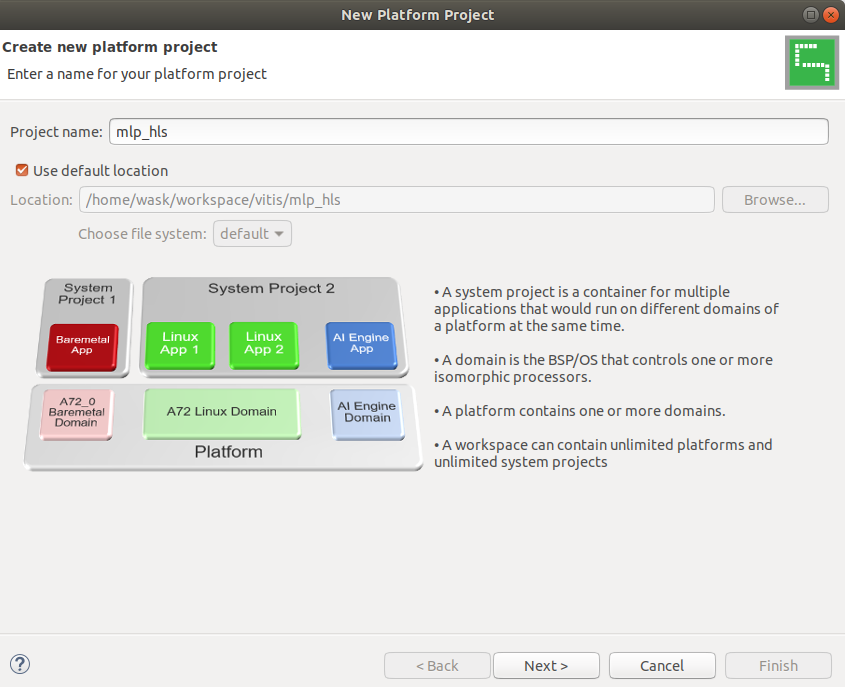
\includegraphics[width=0.9\textwidth]{img/new-vitis-project1.png}
  \caption{Tworzenie nowego projektu w programie Vitis}
  \label{new-vitis-project1}
\end{figure}


\begin{figure}[!h]
  \centering
  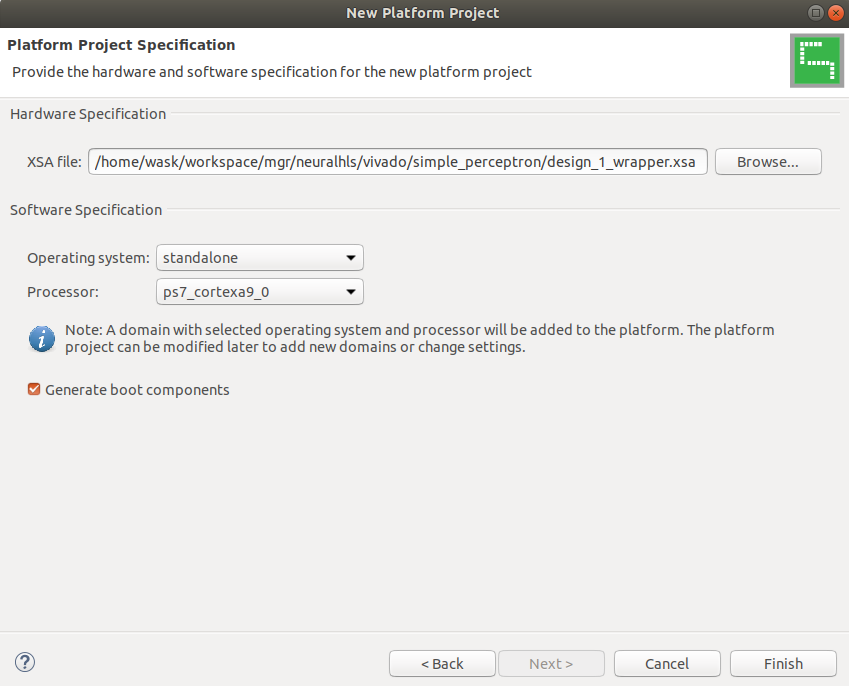
\includegraphics[width=0.9\textwidth]{img/new-vitis-project2.png}
  \caption{Wybór pliku .xsa z opisem konfiguracji sprzętu w programie Vitis}
  \label{new-vitis-project2}
\end{figure}

Następnie należy stworzyć projekt aplikacji, za pomocą opcji \emph{New Application Project} i wybraniu odpowiedniego, 
stworzonego wcześnie projektu platformy. Narzędzie Vitis zawiera szereg aplikacji przykładowych, z których warto 
skorzystać przy uruchamianiu systemu po raz pierwszy. Przed zbudowaniem projektu, aby zapewnić komunikację płytki 
Z-turn Board z komputerem za pomocą konwertera USB-UART znajdującego się na płytce, należy zmienić następujące 
ustawienia BSP (ang. \emph{Board Support Package}) dla domeny \emph{standalone}:

\begin{itemize}
  \item stdin z ps\_7uart\_0 na ps\_7uart\_1
  \item stdout z ps\_7uart\_0 na ps\_7uart\_1
\end{itemize}

Po zbudowaniu projektu platformy można przejść do pisania kodu aplikacji. Warto zaznaczyć, że do uruchomienia i 
debugowania aplikacji na płytce Z-turn Board, potrzebny jest programator JTAG \emph{Xilinx Platform Cable}. Aby 
obejrzeć wyjście standardowe programu, należy otworzyć okno \emph{Vitis Serial Terminal} i wybrać odpowiedni port USB. 
Trzeba również pamiętać o wybraniu odpowiedniej opcji uruchamiania płytki, poprzez ustawienie zworki na JP1 zwarte i 
JP2 rozwarte.

\begin{figure}[!h]
  \centering
  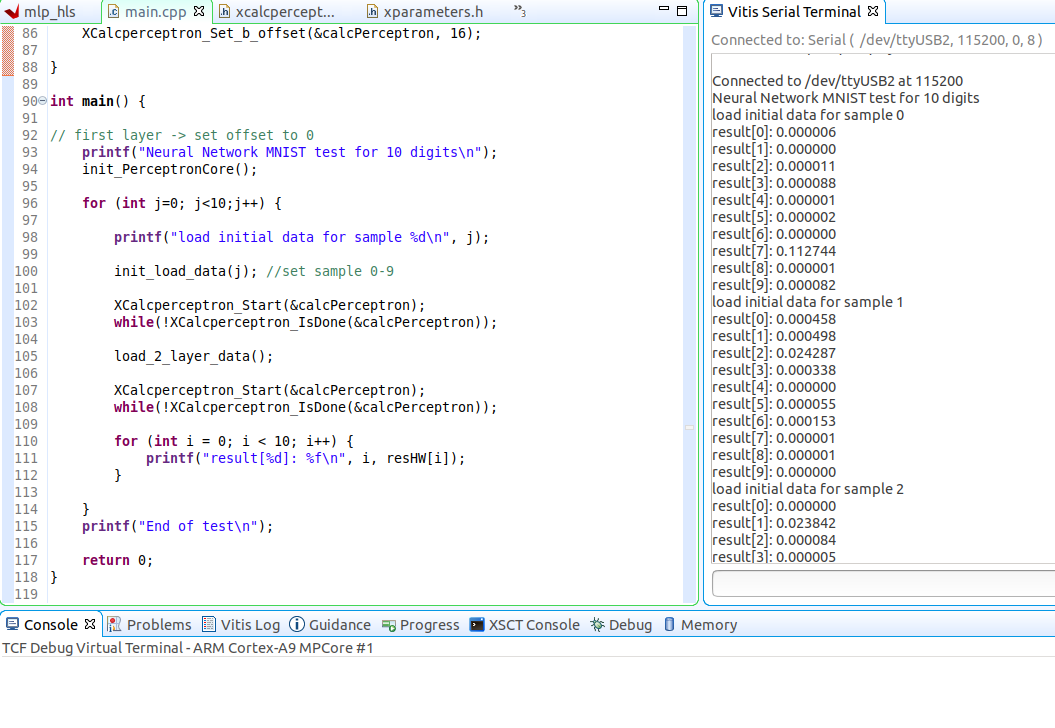
\includegraphics[width=\textwidth]{img/vitis-results.png}
  \caption{Wynik uruchomienia aplikacji w programie Vitis}
  \label{vitis-results}
\end{figure}

Jak widać na Rys. \ref{vitis-results}, algorytm działa poprawnie. Po uruchomieniu i sprawdzeniu poprawności obliczeń w 
programie Vitis można przystąpić do konfigurowania systemu operacyjnego przy użyciu narzędzia Petalinux. 

\subsection{Test z wykorzystaniem systemu operacyjnego Petalinux}

PetaLinux Software Development Kit (SDK) jest narzędziem zawierającym wszystkie niezbędne elementy do budowania,
rozwijania, testowania i wdrażania systemów wbudowanych opartych na systemie Linux. PetaLinux jest przeznaczony głównie 
do systemów, opartych o układy FPGA i składa się z trzech najważniejszych elementów: 

\begin{itemize}
  \item prekonfigurowany obraz binarny systemu 
  \item system Linux konfigurowalny do zastosowania na sprzęcie firmy Xilinx 
  \item PetaLinux SDK zawierający narzędzia służące do projektowania i wdrażania systemu 
\end{itemize}

\subsubsection{Wstępna konfiguracja systemu Petalinux}

Zgodnie z zaleceniami producenta, projekcie wykorzystano wersję narzędzia Petalinux kompatybilną z wersją Vivado -- 
2019.2. Każdorazowo, przed użyciem Petalinuxa należy pamiętać o załadowaniu ustawień przy pomocy komendy:

\begin{verbatim}
  source <katalog-instalacyjny>/petalinux/2019.2/settings.sh
\end{verbatim} 

Narzędzie zużywa dużo przestrzeni dyskowej, jeśli wolnego miejsca będzie zbyt mało, zostanie wyświetlony odpowiedni 
komunikat. Następnie można przejść do tworzenia nowego projektu z ustawieniami domyślnymi dla płytek z układami \emph
{Zynq}:
\begin{verbatim}
  petalinux-create -t project -n <nazwa_projektu> --template_zynq
\end{verbatim}

Projekt sprzętu w programie Vivado został wyeksportowany do pliku z rozszerzeniem \emph{.xsa}. Aby zaimportować plik opisujący konfigurację sprzętu, utworzonego w programie Vivado stosujemy następującą komendę:

\begin{verbatim}  
  petalinux-config --get-hw-description <katalog_projektu_vivado>
\end{verbatim}

Po wywołaniu komendy \emph{petalinux-config} pojawia się interfejs graficzny narzędzia Petalinux, który umożliwia 
zmianę ogólnych ustawień projektu (Rys. \ref{petalinux-config}). Przechodząc do zakładki \emph{Image Packaging 
Configuration} (Rys. \ref{petalinux-config}), można ustawić lokalizację zewnętrznego systemu plików oraz wybrać 
partycję karty sd, na której będzie się znajdował. Stosując opcję -c komendy \emph{petalinux-config} można dostosować 
ustawienia jądra Linuxa (argument \emph{kernel}) oraz systemu plików (argument \emph{rootfs}).

\begin{figure}[!h]
  \centering
  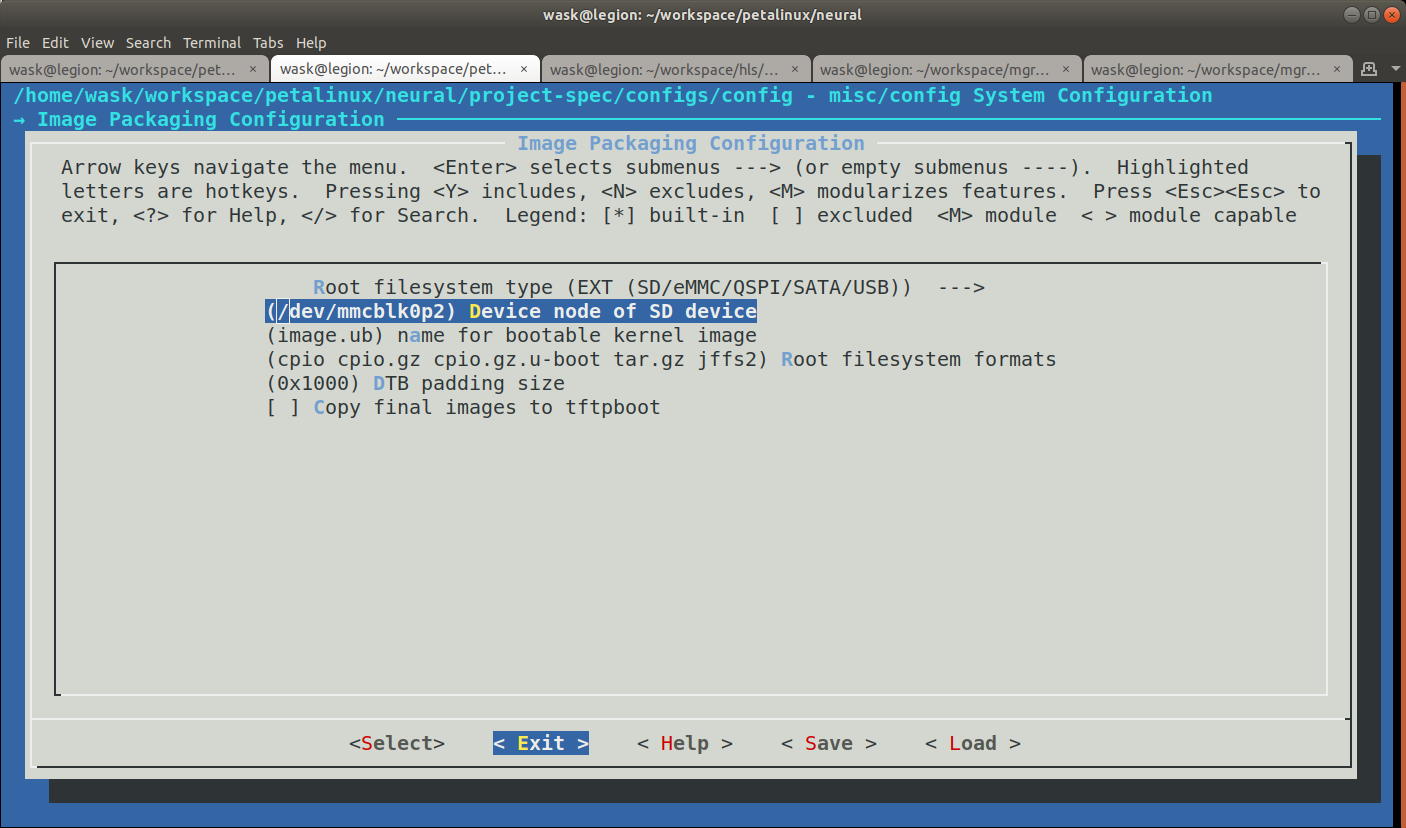
\includegraphics[width=\textwidth]{img/petalinux-config.png}
  \caption{Wstępna konfiguracja przy użyciu funkcji petalinux-config}
  \label{petalinux-config}
\end{figure}

\subsubsection{Konfiguracja jądra systemu Petalinux}

Po wywołaniu komendy \emph{petalinux-config -c kernel} w terminalu pojawia się menu konfiguracyjne jądra systemu 
Petalinux. W oknie jest wiele opcji, jednak najwięcej zmian wprowadzono w zakładce \emph{Device Drivers}. 

W projekcie podjęto decyzję o zastosowaniu kamery podłączonej przy użyciu portu USB. Aby umożliwić aplikacji 
korzystającej z biblioteki OpenCV dostęp do urządzenia, potrzebne były odpowiednie sterowniki \cite{usb-camera} 
dostępne w zakładce \emph{Multimedia Support}. Zastosowany w projekcie moduł kamery MY-CAM002U jest kompatybilny ze 
sterownikiem UVC (ang. \emph{USB Video Class}). W konfiguracji jądra dodano również interfejs V4L2, który daje dostęp 
do modułu kamery z poziomu aplikacji z przestrzeni użytkownika.

\begin{figure}[!h]
  \centering
  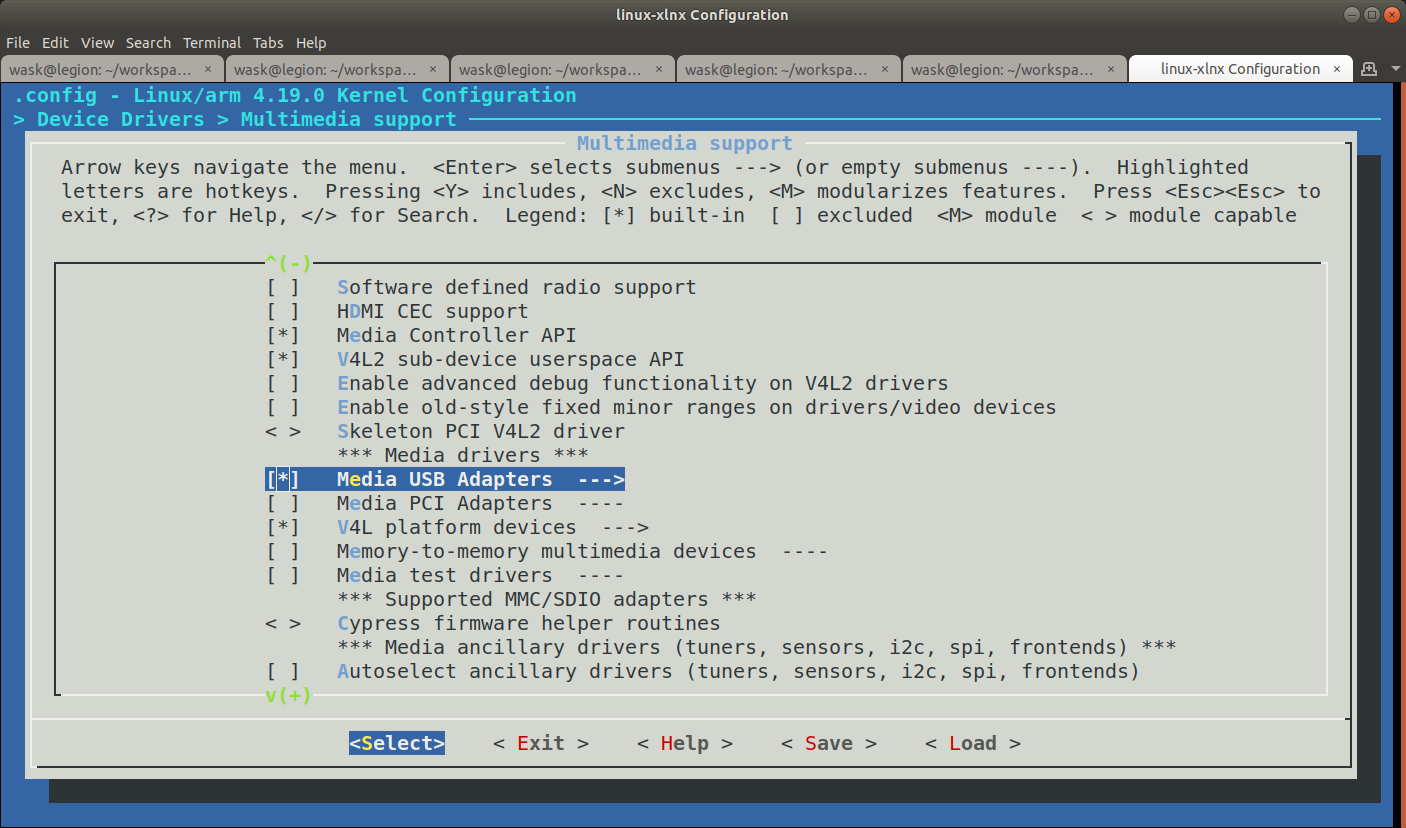
\includegraphics[width=\textwidth]{img/petalinux-config-kernel.png}
  \caption{Konfiguracja jądra PetaLinuxa}
  \label{petalinux-config-kernel}
\end{figure}

Aby uzyskać dostęp z poziomu systemu Petalinux do bloku IP zaimplementowanego w~narzędziu Vivado HLS, należy 
zainstalować odpowiednie sterowniki urządzeń lub utworzyć własne. Dla wielu typów urządzeń tworzenie nowego sterownika 
nie jest konieczne. Alternatywnym rozwiązaniem jest zastosowanie sterownika UIO (ang. \emph{Userspace Input Output 
Driver}) \cite{uio-drivers}, który umożliwia dostęp do urządzenia w aplikacji z przestrzeni użytkownika. Znacznie 
upraszcza to proces tworzenia oprogramowania do obsługi urządzenia i zmniejsza ryzyko powstawania trudnych w 
debugowaniu i często niebezpiecznych dla działania systemu operacyjnego błędów. Jednak należy pamiętać, że sterowniki 
UIO nie są przeznaczone dla dowolnego typu sprzętu. Stosuje się je do obsługi urządzeń, generujących przerwania, 
posiadających pamięć, którą można zmapować i sterować urządzeniem poprzez pisanie do tej pamięci. 

\subsubsection{Konfiguracja systemu plików}

Narzędzie Petalinux umożliwia również dostosowanie systemu plików do potrzeb użytkownika. W menu konfiguracyjnym jest 
wiele pakietów i bibliotek do różnych zastosowań. W zakładce \emph{apps} użytkownik ma dostęp do aplikacji, które 
stworzył w obrębie danego projektu. Narzędzie Petalinux umożliwia utworzenie nowej aplikacji przy użyciu komendy:
\begin{verbatim}
  petalinux-create -t apps -n <nazwa_aplikacji>
\end{verbatim}.

W projekcie zdecydowano się na użycie skryptów napisanych w języku Python i biblioteki OpenCV do rejestrowania obrazu i 
wysyłania go poprzez port Ethernet do komputera PC. W tym celu zaznaczono następujące opcje w konfiguracji systemu 
plików:  

\begin{itemize}
  \item python i python-math
  \item python-numpy
  \item packagegroup-petalinux-v4lutils 
  \item packagegroup-petalinux-opencv
\end{itemize}


Kolejnym etapem w procesie konfigurowania systemu Petalinux jest dostosowanie drzewa urządzeń (ang. \emph{device-tree}
. Drzewo urządzeń można edytować za pomocą plików system-user.dtsi oraz pl-custom.dtsi dostępnych w katalogu:

\begin{verbatim}
  <katalog_projektu>/project-spec/meta-user/recipes-bsp/device-tree
\end{verbatim}
W przypadku wykorzystania sterowników UIO należy wpisać w polu \emph{compatible} każdego z~węzłów urządzeń (pamięci 
BRAM) wartość \emph{"generic-uio"} \cite{uio-device-tree}. Dostęp do urządzeń jest zapewniony dzięki plikom /dev/uioX, 
gdzie X to numer urządzenia (zaczynając od 0 dla pierwszego urządzenia).

\subsubsection{Przygotowanie obrazu systemu}

Po dostosowaniu pliku \emph{device-tree} można uruchomić kompilację petalinuxa komendą \emph{petalinux-build}.
Gdy system zostanie zbudowany, należy spakować wszystkie potrzebne pliki przy użyciu funkcji \emph{petalinux-package}.
Wynikiem tej operacji są dwa pliki dostępne w~katalogu images/linux BOOT.bin i image.ub, które należy przekopiować na
odpowiednią partycję karty sd. Jeśli w konfiguracji Petalinuxa wyłączona została opcja wspierania Initial RAM
filesystem, należy dodatkowo wypakować system plików na drugiej partycji na karcie~sd. Tak przygotowaną kartę sd można
umieścić w slocie na płytce Z-turn, podłączyć zasilanie i uruchomić system.Istnieje opcja kompilacji jedynie wybranej 
aplikacji stworzonej przez użytkownika przy pomocy komendy \emph{petalinux-build -c <nazwa\_aplikacji>}. W~przypadku 
wprowadzenia zmian w systemie, przed ponownym wypakowaniem systemu plików, należy sformatować partycję zawierającą 
system plików. 

\subsubsection{Uruchomienie systemu Petalinux}

Komunikacja płytki Z-turn z komputerem PC odbywa się na dwa sposoby:
\begin{itemize}
  \item przez interfejs UART przy użyciu aplikacji Minicom (Rys. \ref{petalinux-boot})
  \item przez port Ethernet za pomocą kilenta SSH 
\end{itemize}
Oba rozwiązania były stosowane równolegle na każdym etapie projektu. 

\begin{figure}[!h]
  \centering
  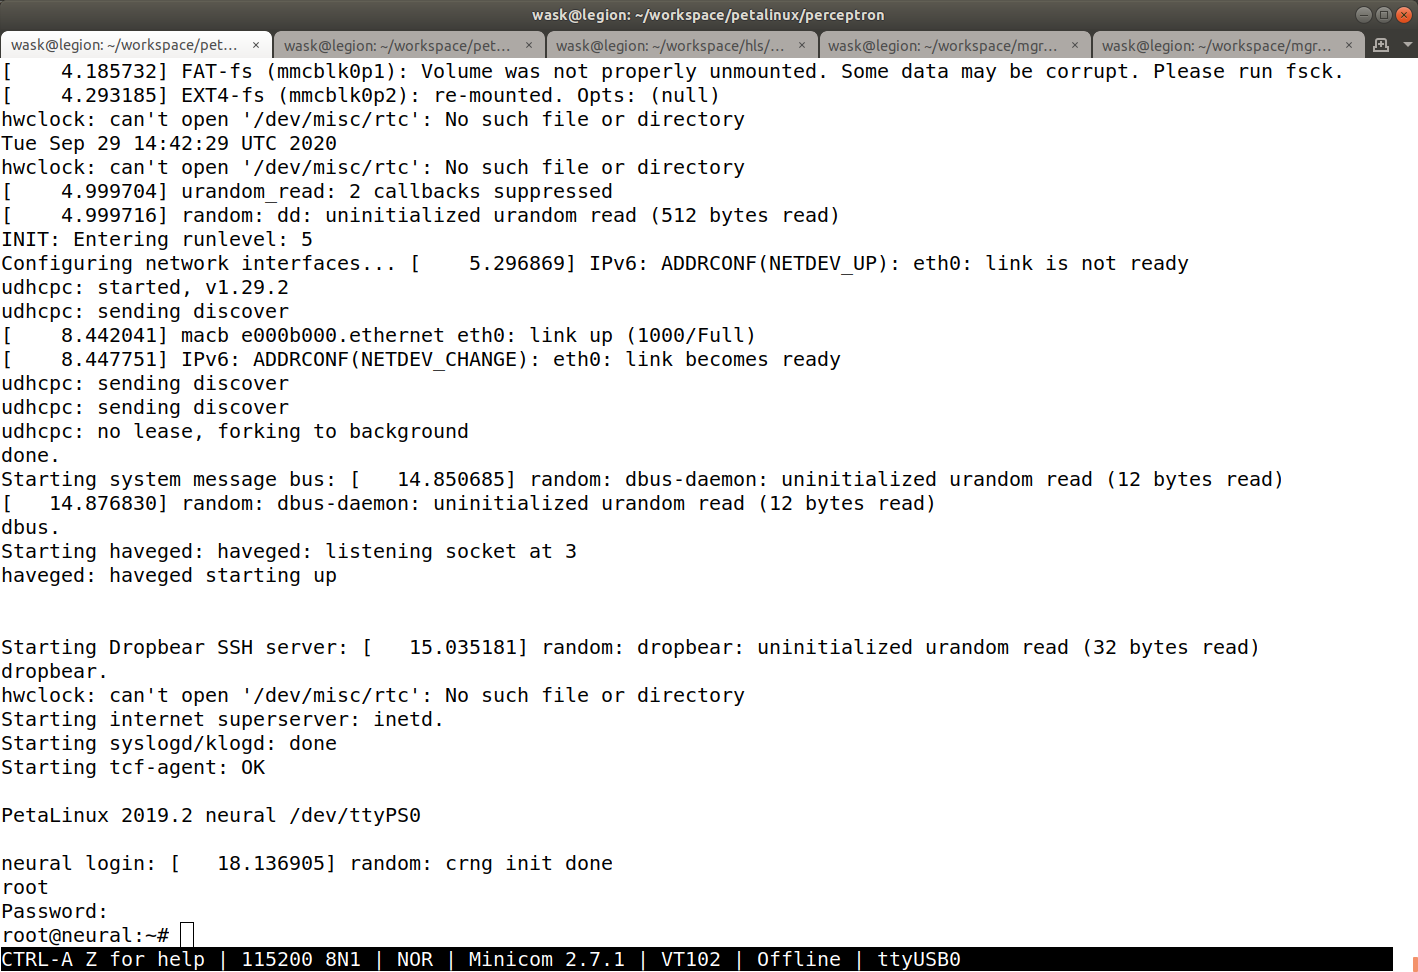
\includegraphics[width=\textwidth]{img/petalinux-boot.png}
  \caption{Uruchomienie systemu PetaLinux}
  \label{petalinux-boot}
\end{figure}

Zaletą konsoli podłączonej za pomocą portu szeregowego jest to, że są w niej wyświetlane komunikaty jądra Linuxa. Ułatwia to debugowanie błędów, które pojawiają się w~fazie uruchamiania systemu operacyjnego. Zaletą protokołu SSH jest duża przepustowość i możliwość wysyłania nawet dużych plików.


